\chapter{playback engine}
\renewcommand{\baselinestretch}{\mystretch}
\label{chap:Playback}
%\setlength{\parindent}{0pt}

\section{Implementation and optimisation}

After verified the ability of loading and rendering the exported lighting sequence by controller dedicated implementations, the C\# code for loading exported sequence was integrated into Vixen application as a separate playback engine. Several code branches were added to switch between the original execution engine and the new playback engine. The execution engine was still used as the default engine to simplify status checking and support the sequence editor. The playback engine will only be switched to if it has started rendering sequence.

The playback engine starts by reading the exported network XML file. To simplify the process, XML object serialiser was used to interpret the XML file to a similarly structured object for later access. The information from XML will be used to determine controller channel mapping, update interval and optional audio media file. To further reduce overhead, the controller names will be looked up and converted to their unique ID (GUID) for later lookup. The optional audio media file was supported by utilising the same audio media functions from original execution engine.

All preview, element and filter updates were skipped in the playback engine. The translation layers were skipped, since the sequence data is already specific to the controllers. However, in order to match the existing interface of controller modules, the sequence data still need to be copied again to specific command types, incurred some unnecessary overhead.

The structure of update management was also changed. Previously, the application updates the channel data buffer from any controller update request, which requires the use of mutex to lock data access between controller threads. With a configuration of multiple controllers, the possible race condition of the mutex can also incur some overhead. Another thread dedicated to sequence loading was add to the playback engine to address this issue, similar to the structure of controller specific implementations. In this way, only the sequence loading thread may update the channel data buffer, removed the need of mutex locker.

One major drawback of using the playback engine is that the data dump cannot be mapped back to element states yet. Therefore, editing the sequence using the built-in editor and the preview output were not supported.

\section{Integration}

A simple control dialog was added as a menu entry for the preview engine, as shown by \fref{fig:vixen_playback}. More complex and user-friendly UI design is possible, however, due to limited time constraint this control dialog should be sufficient for this project and proof of concept.

\begin{figure}[t]
  \centering
  \includegraphics[width=0.8\columnwidth]{Figs/vixen_playback.png}
  \caption{Screenshot of the playback engine controller}
  \label{fig:vixen_playback}
\end{figure}

The playback control was also integrated with built-in schedulers. It can therefore be scheduled to execute multiple times at specific time, possibly with schedules using the original execution engine. The new playback engine does not need additional pre-process for show schedules, can be directly started within seconds.

\section{Performance}

\fref{fig:playback} shows the performance of the playback engine using a ``Raw'' sequence dump. At the first and the last few seconds, the playback engine stopped, the original execution engine was used instead during idle state. However, the execution engine still uses around $30 \%$ of CPU time during idle. But as soon as playback started, CPU usages drops to around $6 \%$ with stable refresh frame rates.

\begin{figure}[t]
  \centering
  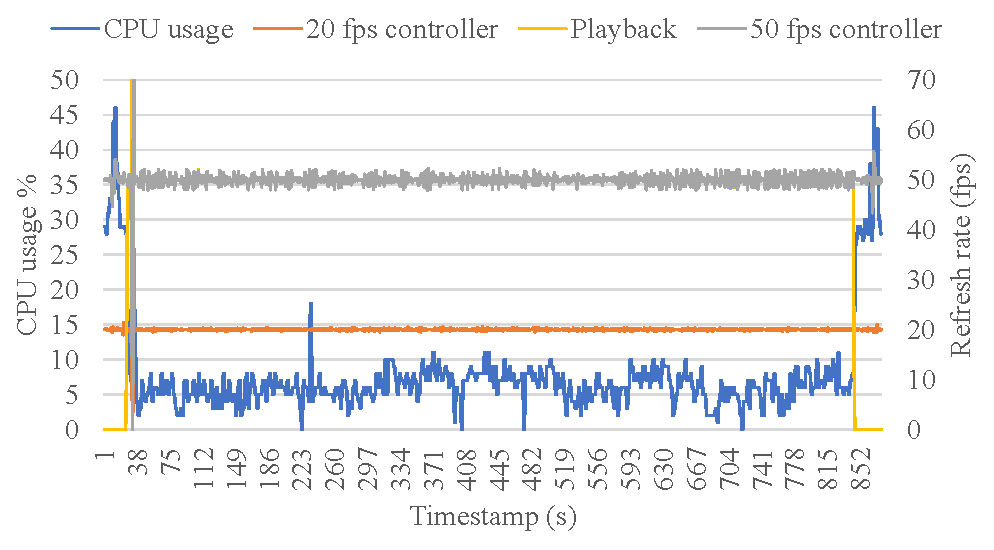
\includegraphics[width=0.8\columnwidth]{playback}
  \caption{Performance of new playback engine}
  \label{fig:playback}
\end{figure}
